\section[Choix 1 des coefficients de la CI3]{Choix des coefficients de la CI3 par moindres carrés sur l'impédance}

  Dans la section précédente, nous avons exprimé les matrices \(\hat\mZ\) et la matrice \(\hat\mR\) en fonction de l'empilement.
  Nous allons montrer que nous pouvons choisir deux manières de calculer les coefficients de la CIOE CI3 (ce qui s'etend facilement au CIOE dérivées de cette dernière). 

  % On se donne \(N_x\) \(k_x\) et \(N_y\) \(k_y\).
  % Il existe donc \(N_k=N_xN_y\) couples tels que \((k_{xi},k_{yj}) = (k_x,k_y)_{(j-1)N_x+i}\).
  \begin{defn}
    Soit \(\ps{\cdot}{\cdot}\) le produit scalaire usuel de \(\CC^{N_{k}}\) et \(\norm{\cdot}\) la norme associée.
    \begin{equation*}
      \ps{a}{b} = \sum_{i=1}^{N_k} \conj{a_i} b_i.
    \end{equation*}
    Soit \(\ps{\cdot}{\cdot}_F\) le produit scalaire usuel de \(\mathcal{M}_2(\CC)\) et \(\norm{\cdot}_F\) la norme associée.
    \begin{equation*}
      \ps{\mA}{\mB}_F = \operatorname{Tr}(\conj{\mA^t}\mB).
    \end{equation*}
  \end{defn}

  \subsection{Calcul des coefficients pour une incidence}

    \begin{defn}
      On définit \(\mH_{CI3}\) la fonction de \(\RR \times \RR \times \mathcal{M}_2(\CC) \rightarrow \mathcal{M}_{4\times5}(\CC)\) telle que
      \begin{equation*}
        \mH_{CI3}(k_x,k_y,\mZ) = \begin{bmatrix}
        1 & \hat{\mLD}(k_x,k_y)_{11} & -\hat{\mLR}(k_x,k_y)_{11} & -\left(\hat{\mLD}(k_x,k_y)\mZ\right)_{11} & \left(\hat{\mLR}(k_x,k_y)\mZ\right)_{11}
        \\
        0 & \hat{\mLD}(k_x,k_y)_{12} & -\hat{\mLR}(k_x,k_y)_{12} & -\left(\hat{\mLD}(k_x,k_y)\mZ\right)_{12} & \left(\hat{\mLR}(k_x,k_y)\mZ\right)_{12}
        \\
        0 & \hat{\mLD}(k_x,k_y)_{21} & -\hat{\mLR}(k_x,k_y)_{21} & -\left(\hat{\mLD}(k_x,k_y)\mZ\right)_{21} & \left(\hat{\mLR}(k_x,k_y)\mZ\right)_{21}
        \\
        1 & \hat{\mLD}(k_x,k_y)_{22} & -\hat{\mLR}(k_x,k_y)_{22} & -\left(\hat{\mLD}(k_x,k_y)\mZ\right)_{22} & \left(\hat{\mLR}(k_x,k_y)\mZ\right)_{22}
        \end{bmatrix}.
      \end{equation*}
      On définit \(b\) la fonction de \(\mathcal{M}_2(\CC) \rightarrow \CC^4\) telle que
      \begin{equation*}
        b(\mZ) = \begin{bmatrix}
        \mZ_{11}
        \\
        \mZ_{12}
        \\
        \mZ_{21}
        \\
        \mZ_{22}
        \end{bmatrix}.
      \end{equation*}
    \end{defn}

    \begin{prop}
      Soit \(X = (a_0,a_1,a_2,b_1,b_2)\), \((k_x,k_y)\) fixé et \(\hat\mZ_{ex}\) l'opérateur d'impédance exact du plan, alors
      \begin{multline*}
        \argmin{X\in\CC^5} \norm{\hat\mZ_{CI3}(k_x,k_y,X) - \hat\mZ_{ex}(k_x,k_y)} =
        \\
        \argmin{X\in\CC^5} \norm{\mH_{CI3}(k_x,k_y,\hat\mZ_{ex}(k_x,k_y))X - b(\hat\mZ_{ex}(k_x,k_y))}.
      \end{multline*}
    \end{prop}

    \begin{proof}
      On rappelle que dans la section précédente, on a introduit
      \begin{multline*}
        \hat{\mZ}_{CI3}(k_x,k_y) = \left(\mI + b_1 \hat{\mLD}(k_x,k_y) - b_2 \hat{\mLR}(k_x,k_y) \right)^{-1}\\\left(a_0 \mI + a_1 {\hat{\mLD}(k_x,k_y)} - a_2 {\hat{\mLR}(k_x,k_y)}\right).
      \end{multline*}
      On pose
      \begin{align*}
        \hat\mZ_D(k_x,k_y) &= \mI + b_1 \hat{\mLD}(k_x,k_y) - b_2 \hat{\mLR}(k_x,k_y),
        \\
        \hat\mZ_N(k_x,k_y) &= a_0 \mI + a_1 {\hat{\mLD}(k_x,k_y)} - a_2 {\hat{\mLR}(k_x,k_y)}.
      \end{align*}

      Et ainsi, on développe
      \begin{align*}
      &{}~ \argmin{X\in\CC^5} \norm{\hat\mZ_{CI3}(k_x,k_y,X) - \hat\mZ_{ex}(k_x,k_y)}
      \\
      & = \argmin{X\in\CC^5} \norm{\hat\mZ_D(k_x,k_y)^{-1}\hat\mZ_N(k_x,k_y) - \hat\mZ_{ex}(k_x,k_y) },
      \\
      &= \argmin{X\in\CC^5} \norm{\hat\mZ_D(k_x,k_y)^{-1}\left(\hat\mZ_N(k_x,k_y) - \hat\mZ_D(k_x,k_y)\hat\mZ_{ex}(k_x,k_y)\right) },
      \\
      &= \argmin{X\in\CC^5} \norm{\hat\mZ_N(k_x,k_y) - \hat\mZ_D(k_x,k_y)\hat\mZ_{ex}(k_x,k_y)},
      \\
      &= \argmin{X\in\CC^5} \norm{\hat\mZ_N(k_x,k_y) - \left(b_1 \hat{\mLD}(k_x,k_y) - b_2 \hat{\mLR}(k_x,k_y)\right)\hat\mZ_{ex}(k_x,k_y) - \hat\mZ_{ex}(k_x,k_y) },
      \\
      &= \argmin{X\in\CC^5} \norm{\mH_{CI3}(k_x,k_y,\hat\mZ_{ex}(k_x,k_y))X - b(\hat\mZ_{ex}(k_x,k_y))}.
      \end{align*}
    \end{proof}

    Les fonctions associées aux CIOE CI0, CI01, CI1, CI4 se déduisent aisément.

    Pour un couple \((k_x,k_y)\), les coefficients d'une CIOE (ici la CI3) sont solutions d'un problème d'optimisation.
    Cependant, comme sans pertes de généralités, nous pouvons nous ramener à des matrices diagonales quand \(k_y\) est nul, alors il existera une infinité de solution possible.
    % Cependant, ces coefficients deviennent donc fonction de cette "incidence". 
 
    % Pour compléter, voici \(\mH_{CI1}\) la fonction de \(\RR \times \RR \times \mathcal{M}_2(\CC) \rightarrow \mathcal{M}_{4\times3}(\CC)\) telle que
    % \begin{equation*}
    %   \mH_{CI1}(k_x,k_y,\mZ) = 
    %   \begin{bmatrix}
    %     1 & -(k_x^2+k_y^2)  & \left(k_x^2+k_y^2\right)\mZ_{11}
    %     \\
    %     0 & 0               & \left(k_x^2+k_y^2\right)\mZ_{12}
    %     \\
    %     0 & 0               & \left(k_x^2+k_y^2\right)\mZ_{21}
    %     \\
    %     1 & -(k_x^2+k_y^2)  & \left(k_x^2+k_y^2\right)\mZ_{22}
    %   \end{bmatrix}.
    % \end{equation*}


  \subsection{Balayage en incidences et moindres carrés}

    Pour déterminer numériquement les coefficients de la CIOE, nous allons considérer que \(k_x,k_y\) appartient respectivement à un domaine discret réel de taille respectivement \(N_{k_x}, N_{k_y}\).

    \begin{defn}
      On définit \(\mA_{CI3}\) la matrice de \(\mathcal{M}_{4N_xN_y\times5}(\CC)\) telle que
      \begin{equation*}
        \mA_{CI3} = 
        \begin{bmatrix}
          \mH_{CI3}(k_{x1},k_{y1},\hat\mZ_{ex}(k_{x1},k_{y1}))
          \\
          \vdots
          \\
          \mH_{CI3}(k_{xi},k_{yj},\hat\mZ_{ex}(k_{xi},k_{yj}))
          \\
          \vdots
          \\
          \mH_{CI3}(k_{xN_x},k_{yN_y},\hat\mZ_{ex}(k_{xN_x},k_{yN_y}))
        \end{bmatrix}.
      \end{equation*}
      On définit \(g\) la vecteur colonne complex tel que
      \begin{equation*}
        g = 
        \begin{bmatrix}
          b(\hat\mZ_{ex}(k_{x1},k_{y1}))
          \\
          \vdots
          \\
          b(\hat\mZ_{ex}(k_{xi},k_{yj}))
          \\
          \vdots
          \\
          b(\hat\mZ_{ex}(k_{xN_x},k_{yN_y}))
        \end{bmatrix}.
      \end{equation*}
    \end{defn}

    \begin{defn}
      On pose \(\mM_{CI}=\conj{\mA_{CI}^t}{\mA_{CI}}\).
    \end{defn}

    Cette matrice est importante car comme nous le montrerons plus tard, elle apparaît dans la forme quadratique associée à la minimisation.
    Nous allons donc démontrer immédiatement que la matrice associée à une des CIOE est inversible.
    Cela nous permettra de démontrer l’existence et l'unicité de la solution du problème de minimisation vérifié par les coefficients de la CIOE.

  \subsection[Inversibilité des matrices Mci]{Inversibilité des matrices \(\mM_{CI}\)}

    \subsubsection{Pour la CI01}

      \begin{prop}
        La matrice \({\mM}_{CI01}\)
        associée à la CI01 est inversible, si et seulement s'il existe au moins deux couples \((k_{x},k_{y})\) différents.
      \end{prop}

      \begin{proof}
        Soit \(t\) le vecteur de \(\RR_+^{N_{k}}\) tel que \(t_{(j-1)N_x+i} = k_{xi}^2 + k_{yj}^2\) et \(1\) le vecteur de \(\RR^{N_{k}}\) dont tous les éléments sont \(1\). On a l'expression suivante de \({\mM}\)

        \begin{equation*}
          {\mM}_{CI01} = 2\begin{bmatrix}
          N_{k} & -\sum_{i=1}^{N_{k}} t_i
          \\
          -\sum_{i=1}^{N_{k}} t_i & \sum_{i=1}^{N_{k}} t_i^2
          \end{bmatrix}
          = 2\begin{bmatrix}
          \ps{1}{1} & -\ps{1}{t}
          \\
          -\ps{t}{1} & \ps{t}{t}
          \end{bmatrix}.
        \end{equation*}
        Pour prouver son inversibilité, on exprime son déterminant 
        \begin{align*}
          %\det( {\mM}_{CI01}) &= 4\left(N_{k}\sum_{i=1}^{N_{k}} t_i^2 - \left( \sum_{i=1}^{N_{k}} t_i\right)^2\right),
          %\\
           &= 4\left( \ps{1}{1}\ps{t}{t} - \ps{t}{1}^2\right).
        \end{align*}
        Donc d'après Cauchy–Schwarz (voir \cite[\href{https://dlmf.nist.gov/1.7\#E1}{eq.~1.7.1}]{dlmf_nist_2019}), le terme de droite est non-nul pour tout \(t\) non colinéaire au vecteur dont toutes les composantes valent 1, c'est-à-dire n'importe quel vecteur ayant au moins deux composantes différentes.
      \end{proof}

    \subsubsection{Pour la CI4}

      \begin{prop}
        La matrice \({\mM}_{CI4}\)
        associée à la CI4 est inversible, si et seulement s'il existe au moins deux couples \((k_{xi},k_{yi})\) différents.
      \end{prop}

      \begin{proof}
        En reprenant la définition des vecteurs de \(\RR_+^{N_{k}}\) \(t\) et \(1\) introduits ci-avant, on a
        \begin{equation*}
          {\mM}_{CI4} = \begin{bmatrix}
          2\ps{1}{1} & -\ps{1}{t} & -\ps{1}{t}
          \\
          -\ps{t}{1} & \ps{t}{t}  & 0
          \\
          -\ps{t}{1} & 0          & \ps{t}{t}
          \end{bmatrix}.
        \end{equation*}
        Donc immédiatement
        \begin{align*}
          \det({\mM}_{CI4}) &= 2\ps{t}{t}\left( \ps{1}{1}\ps{t}{t} - \ps{t}{1}^2\right).
        \end{align*}
        On conclu ici-aussi grâce à Cauchy–Schwarz.
      \end{proof}

      \subsubsection{Pour la CI1}

      L'introduction de \(\hat\mZ_{ex}\) dans \(\mM\) ne permet plus d'exprimer simplement le déterminant de cette dernière. 
      Nous n'avons pas réussi à prouver que \(\det({\mM}_{CI1})\) est inversible.

      Cependant nous avons vérifié numériquement qu'elles l'étaient pour tous les empilements que nous avons testés.

      Nous pouvons néanmoins exprimer la matrice et le déterminant et l'inversibilité reste une perspective.

      Nous renvoyons aux définitions des vecteurs de \(\RR_+^{N_{k}}\) \(t\) et \(1\) introduits ci-avant.

      Soient \(s\) le vecteur de \(\CC^{N_{k}}\) tel que \(s_i = \ps{\mI}{\hat{\mZ}(k_{x},k_{y})_i}_F\) et \(z\) le vecteur de \(\RR^{N_{k}}\) tel que \(z_i = \norm{\hat{\mZ}(k_{x},k_{y})_i}_F\). On a l'expression suivante de \({\mM_{CI1}}\)

      \begin{equation*}
        {\mM}_{CI1} = \begin{bmatrix}
        2\ps{1}{1}  & -2\ps{t}{1} & \ps{t}{s}
        \\
        -2\ps{t}{1} & 2\ps{t}{t} & -\sum_{i=1}^{N_{k}} t_i^2 s_i
        \\
        \ps{t}{\conj{s}} & -\sum_{i=1}^{N_{k}} t_i^2 \conj{s_i} & \sum_{i=1}^{N_{k}} t_i^2 z_i^2 
        \end{bmatrix}.
      \end{equation*}
      
      Alors 
      \begin{multline*}
        \det( {\mM}_{CI1}) = \ps{t^2}{z^2}\det({\mM}_{CI01}) + 4 \ps{t}{1}\Re\left(\ps{t^2}{s}\ps{t^2}{\conj{s}}\right)
        \\
        - 2\norm{t}^2|\ps{t}{s}|^2 - 2 N_k|\ps{t^2}{s}|^2.
      \end{multline*}

    \begin{REM}
      Sois positif : "numériquement, nous avons toujours eu l'inversibilité, mais nous savons que cette dernière n'est pas inconditionnelle, ex 2 angles."...
    \end{REM}

      \begin{REM}
        J'ai fais le cas \(N_k=2\).
        \begin{multline*}
          det = 4(t_1-t_2)^2(t_1^2z_1+t_2^2z_2)
          \\
          + 2t_1t_2(t_1-t_2)(\conj{s_1}-\conj{s_2})(t_1s_1+t_2s_2)
          \\
          +2(t_1-t_2)(t_1^2s_1+t_2^2s_2)(\conj{s_2}t_2-\conj{s_1}t_1)
        \end{multline*}
        sauf erreur de calcul.
        Obtenue en utilisant \(2t_1 = t_1 + t_2 + t_1 - t_2\), \(2t_2 = t_1 + t_2 - (t_1 - t_2)\)
      \end{REM}
      \begin{REP}
        En effet tu montres que si \(t_1=t_2\), alors det = 0, mais on le sait pour Nk quelconque:

        Supposons t et 1 colinéaires . donc la deuxième colonne est multiple de la première par la valeur d'une des composantes de t.
        Donc il faut nécessairement aux moins 2 ti differents.
        Intuition: au moins 3 pour la CI1
      \end{REP}

      \begin{REP}
        Nouvelle idée, voir CI3.

        On rappelle que  \(\hat\mL(k_x,k_y)=-(k_x^2+k_y^2)\mI\). On remarque que \(t_i = \ps{\mI}{\hat\mL}_F/\ps{\mI}{\mI}_F\).

        Soit \(s\) le vecteur de \(\CC^{N_{k}}\) tel que \(s_i = \ps{\hat\mL(k_{x},k_{y})_i}{\hat{\mZ}(k_{x},k_{y})_i}_F\) et \(l\) le vecteur de \(\RR^{N_{k}}\) tel que \(l_i = \norm{\hat\mL(k_{x},k_{y})_i\hat{\mZ}(k_{x},k_{y})_i}_F\).
        
        On a l'expression suivante de \({\mM_{CI1}}\)

        \begin{equation*}
          {\mM}_{CI1} = \begin{bmatrix}
          2\ps{1}{1}        & -2\ps{t}{1}       & \ps{1}{s}
          \\
          -2\ps{t}{1}       & 2\ps{t}{t}        & -\ps{t}{s}
          \\
          \ps{1}{\conj{s}}  & -\ps{t}{\conj{s}} & \ps{l}{l}
          \end{bmatrix}.
        \end{equation*}
        Finalement pas mieux.

      \end{REP}

      \begin{REP}
        Nouveau: Passons par les noyaux. 

        La matrice M est une somme de matrices de det = 0:
        \begin{align*}
          \mM_{CI1} = \sum_{i=1}^{N_k}
          \begin{bmatrix}
          2  & -2t_i & t_is_i
          \\
          -2t_i & 2t_i^2 & - t_i^2 s_i
          \\
          t_i\conj{s_i} & -t_i^2 \conj{s_i} & t_i^2 z_i^2 
          \end{bmatrix}.
        \end{align*}

        Si l'on peut prouver que les noyaux ne s'intersectent qu'en 0, alors la matrice totale est inversible.

        En effet s'il existe \(\mA\),\(\mB\), et \(x\not=0\) tels que \(\mA x  + \mB x = 0 \), alors soit \(\mA\) est inversible et alors \(x=-\mA^{-1}\mB x\) donc \(\mB= - \mA\) donc \(\mB\) est inversible aussi ( et \(\mA+\mB\equiv 0\) ), soit \(\mA\) n'est pas inversible, donc \(\mA x= 0\), donc \( 0 + \mB x = 0 \), donc \(x\) appartient aussi au noyau de \(\mB\).


        On a alors les cas selon si \(|s_i|^2=2z_i^2\), c'est à dire si \(|\hat\mZ((k_x,k_y)_i)_{11} + \hat\mZ((k_x,k_y)_i)_{22}|^2 = 2 (|\hat\mZ((k_x,k_y)_i)_{11})|^2 + |\hat\mZ((k_x,k_y)_i)_{12})|^2 + |\hat\mZ((k_x,k_y)_i)_{21})|^2 + |\hat\mZ((k_x,k_y)_i)_{22})|^2)\).

        \begin{enumerate}
          \item \(|s_i|^2\not=2z_i^2 \)

          Le noyau est de dim 1 de vecteur \((-t_i,1,0)\) alors il faut que le nombre de \(t_i\) différents soit supérieur à la dimension de la matrice donc 3.
          \item \(|s_i|^2=2z_i^2 \)

          Cela arrive si \(\hat\mZ((k_x,k_y)_i)\) est multiple de l'identité, par exemple \((k_x,k_y)=(0,0)\) car \(\hat\mZ(0,0)=i\eta_r\tan(kd)\mI\).

          Le noyau est de dimension 2, \((-t_i,1,0)\),\((1/2t_i\conj{s_i},0,1)\). 

          En cours ...

        \end{enumerate}


      \end{REP}

    \subsubsection{Pour la CI3}

      Nous n'avons pas réussi à démontrer que cette matrice, associée à la CIOE CI3, était définie pour tout empilement et toute incidence.
      \begin{REM}
        Il faut que tu en dises plus. As-tu trouvé des cas où elle n'est pas inversible ? As-tu fais l'essai avec deux couches ? Est-ce que pour certaines valeurs de \(k_x,k_y\) il y  des cas si \(\eps,\mu\) complexes.
      \end{REM}
      \begin{REP}
        Je n'ai pas trouvé des cas où elle n'est pas inversible et cela n'est pas vérifié fait dans le code mais serait possible.
        Le nombre de couches importe peu : cela n'influe que sur l'expression de \(Z_{ex}\), qui est déjà assez complexe pour une seule couche.
        Le nombre d'incidences a plus d'impact je pense, mais je pense qu'il faut en prendre au moins 3 (intuition).
        C'est une calcul que j'ai tenté plusieurs fois durant ces 3 ans, sans succès.
      \end{REP}

      \begin{REP}
        Nous pouvons néanmoins exprimer la matrice \(\mM_{CI3}\) et son déterminant et l'inversibilité reste une perspective.

        Nous renvoyons aux définitions des vecteurs de \(\RR_+^{N_{k}}\) \(t\) et \(1\) introduits ci-avant.
        Soient \(s_D,s_R\) les vecteurs de \(\CC^{N_{k}}\) et \(l_D,l_R\) les vecteurs de \(\RR_+^{N_{k}}\) tels que
        \begin{align*}
          s_{Di} &= \ps{\mLD(k_{x},k_{y})_i}{\hat{\mZ}(k_{x},k_{y})_i}_F,
          \\
          s_{Ri} &= \ps{\mLR(k_{x},k_{y})_i}{\hat{\mZ}(k_{x},k_{y})_i}_F,
          \\
          l_{Di} &= \norm{\mLD(k_{x},k_{y})_i\hat{\mZ}(k_{x},k_{y})_i}_F,
          \\
          l_{Ri} &= \norm{\mLR(k_{x},k_{y})_i\hat{\mZ}(k_{x},k_{y})_i}_F.
        \end{align*}
        On a l'expression suivante de \({\mM_{CI3}}\)

        \begin{equation*}
          {\mM}_{CI3} = \begin{bmatrix}
          2\ps{1}{1}          & -\ps{t}{1}          & -\ps{t}{1}           & -\ps{1}{s_D}   & \ps{1}{s_R}
          \\
          -\ps{t}{1}          & \ps{t}{t}           & 0                    & \ps{t}{s_D}    & 0
          \\
          -\ps{t}{1}          & 0                   & \ps{t}{t}            & 0              & - \ps{t}{s_R}
          \\
          -\ps{1}{\conj{s_D}} & \ps{t}{\conj{s_D}}  & 0                    & \ps{l_D}{l_D}  & 0
          \\
          \ps{1}{\conj{s_R}}  & 0                   & -\ps{t}{\conj{s_R}}  & 0              & \ps{l_R}{l_R}
          \end{bmatrix}.
        \end{equation*}
        
        % Alors 
        % \begin{multline*}
        %   \det( {\mM}_{CI3}) =
        % \end{multline*}

        % A noter que si on pose

        % \begin{align*}
        %   m_{Di} &= \norm{\mLD\hat{\mZ}(k_{x},k_{y})_i}_F^2
        % \end{align*}
        % alors
        % \begin{equation*}
        %   \ps{l_D}{l_D} = \ps{1}{m_D}
        % \end{equation*}

      \end{REP}
      \begin{REP}
        Par les noyaux.

        Pour alleger les notations, \(\mA((k_x,k_y)_i) = \mA_t\).

        \begin{equation*}
          {\mM}_{CI3} = \sum_{i=1}^{N_k}
          \begin{bmatrix}
          \ps{\mI}{\mI}_F         & \ps{\mI}{\mLD_i}_F       & \ps{\mI}{-\mLR_i}_F          & \ps{\mI}{-\mLD\hat\mZ_i}_F           & \ps{\mI}{\mLR\hat\mZ_i}_F
          \\
          \ps{\mI}{\mLD_i}_F      & \ps{\mLD_i}{\mLD_i}_F    & 0                            & \ps{\mLD}{-\mLD\hat\mZ_i}_F          & 0
          \\
          \ps{\mI}{-\mLR_i}_F     & 0                        & \ps{\mLR_i}{\mLR_i}_F        & 0                                    & \ps{-\mLR}{\mLR\hat\mZ_i}_F
          \\
          \ps{-\mLD\mZ_i}{\mI}_F  & \ps{-\mLD\mZ_i}{\mLD}_F  & 0                            & \ps{\mLD\hat\mZ_i}{\mLD\hat\mZ_i}_F  & 0
          \\
          \ps{\mLR\mZ_i}{\mI}_F   & 0                        & \ps{\mLR\hat\mZ_i}{\mLR}_F   & 0                                    & \ps{\mLR\hat\mZ_i}{\mLR\hat\mZ_i}_F
          \end{bmatrix}.
        \end{equation*}
        
        % Alors 
        % \begin{multline*}
        %   \det( {\mM}_{CI3}) =
        % \end{multline*}

        % A noter que si on pose

        % \begin{align*}
        %   m_{Di} &= \norm{\mLD\hat{\mZ}(k_{x},k_{y})_i}_F^2
        % \end{align*}
        % alors
        % \begin{equation*}
        %   \ps{l_D}{l_D} = \ps{1}{m_D}
        % \end{equation*}

      \end{REP}
  \subsection{Calcul des coefficients des CIOE par moindre carrés}

    \subsubsection[Expression de la fonction JZ]{Expression de la fonction \(J_Z\)}
      On peut alors calculer les coefficients d'une CIOE \(CI\) particulière.
      \begin{defn}
        On définit la fonction \(J_Z\)
        \begin{equation*}
          J_Z(X) = \norm{{\mA}_{CI}X - {g}}^2.
        \end{equation*}
      \end{defn}

    \subsubsection{Minimisation sans contraintes}

      \begin{thm}[Minimisation sans contraintes pour la CI3]
        Les coefficients de la CIOE sont solutions du problème

        Trouver \(X^* \in \CC^N\) tel que
        \begin{equation*}
          X^* = \argmin{X\in \CC^N} J_Z(X).
        \end{equation*}
      \end{thm}

      \begin{proof}
        On remarque que la fonction \(J_Z\) est quadratique si la matrice \(\conj{\mA^t}{\mA}\) est hermitienne définie positive. Une matrice \(\mM\) est hermitienne si \(\forall x, \conj{x^t}\mM x \in \RR\), elle est hermitienne positive si \(\forall x, \conj{x^t}\mM x \in \RR^+\) et elle est hermitienne définie positive si \(\forall x\not=0, \conj{x^t}\mM x \in \RR^{+*}\).

        On remarque que par construction, notre matrice \(\mM\) est hermitienne positive. 
        Dans la section précédente, nous avons démontré l'inversibilité de ces matrices pour des CIOE particulières.

        Dans ce cadre, l'unique minimum est alors solution de \(\vgrads{}J_Z = 0\).
      \end{proof}

      \begin{prop}
        \label{prop:plan:minimisation:minimum_sans_contraintes}
        Si \(\conj{\mA_{CI}^t}\mA_{CI}\) est inversible, alors
        \begin{equation*}
          X^* = (\conj{\mA_{CI}^t}\mA_{CI})^{-1}(\conj{\mA_{CI}^t}g).
        \end{equation*}
      \end{prop}

      \begin{proof}
        \begin{align*}
        J_Z(X) &= \norm{\mA_{CI}X - g}^2,
        \\
        &= \ps{\mA_{CI}X - g}{\mA_{CI}X - g},
        \intertext{le produit scalaire est hermitien donc}
        &=\ps{\mA_{CI}X}{\mA_{CI}X} - \ps{\mA_{CI}X}{g} - \ps{g}{\mA_{CI}X} + \ps{g}{g},
        \\
        &=\ps{X}{\conj{\mA_{CI}^t}\mA_{CI}X} - \ps{X}{\conj{\mA_{CI}^t}g} - \ps{\conj{\mA_{CI}^t}g}{X} + \ps{g}{g},
        \end{align*}
        Si la matrice \(\conj{\mA_{CI}^t}\mA_{CI}\) est inversible, comme elle est par définition hermitienne et positive, alors la fonction est quadratique. Il existe donc un unique minimum où le gradient de cette fonction s'annule. Or
        \begin{align*}
          \nabla J_Z(X^*) &= 2\conj{\mA_{CI}^t}\mA_{CI}X^* - 2\conj{\mA_{CI}^t}g,
          \\ 
          &= 0.
        \end{align*}
      \end{proof}

    \subsubsection{Minimisation avec contraintes}

      \begin{thm}[Minimisation avec contraintes pour la CI3]
        Soit \(\CSU[3]{CI3}\) le sous-espace de \(\CC^5\) issu de la définition \ref{def:csu:ci3-3}.
        Alors les coefficients de la CIOE respectant cette CSU sont solutions du problème.

        Trouver \(X^* \in \CC^5\) tel que
        \begin{equation*}
          X^* = \argmin{X\in \CSU[3]{CI3}}  J_Z(X).
        \end{equation*}
      \end{thm}

      \begin{REM}[minimum]
        Si tu n'as pas de résultats d'existence et unicité, je ne comprends pas ce théorème.
      \end{REM}
      \begin{REP}
        Si l'ensemble des contraintes est convexes, alors il y a existences et unicité. Je n'ai pas sur le montrer pour CI1 et CI3
      \end{REP}

  \subsection{Résultats numériques sans contraintes}

      Sans contraintes, on résout le système linéaire \(\mH X = b\). 
      %Numériquement, nous avons utilisé la routine de résolution au sens des moindres carrés \href{http://www.netlib.org/lapack/explore-html/d6/d10/group__complex16_g_esolve_ga1d8089ba1e1538eb3d1ab0ebe97596c7.html}{ZGELS}.

      Dans \cite{stupfel_implementation_2015} sont introduites les CIOE
      \begin{itemize}
        \item CI01
          \begin{equation*}
            \vE_t = \left(a_0\oI + a_1\frac{\LL}{k_0^2}\right)\vJ,
          \end{equation*}
        \item CI1
          \begin{equation*}
            \left(\oI + b\frac{\LL}{k_0^2} \right)\vE_t = \left(a_0\oI + a_1\frac{\LL}{k_0^2}\right)\vJ.
          \end{equation*}
      \end{itemize}

      L'opérateur \(\LL\) est le laplacien tangentiel \(\lapls\) appliqué à chaque composante. Le multiplicateur de Fourier associé est la matrice.
      \begin{equation*}
        \hat{\mL}  = -
        \begin{bmatrix}
          k_x^2 + k_y^2 & 0
          \\
          0 & k_x^2 + k_y^2
        \end{bmatrix}.
      \end{equation*}

      La matrice \(\mL\) est multiple de l'identité donc la matrice \(\hat\mZ_{CI}\) associée à ces CIOE n'approchera pas bien la matrice \(\hat{\mZ}_{ex}\). La figure \ref{fig:imp_fourier:plan:stupfel:hoibc} présente donc quelques résultats où l'on voit bien la limite de ces CIOE par rapport à la CI3 et il en est de même pour les coefficients de réflexion visible à la figure \ref{fig:reflex_fourier:plan:stupfel:hoibc}.
      \begin{figure}[!hbt]
        \centering
        \tikzsetnextfilename{Z_STUPFEL_plan_hoibc.11}
\begin{tikzpicture}[scale=1]
    \begin{axis}[
            title={Polarisation TM},
            ylabel={\(|\hat{Z}(k_x,0)|\)},
            xlabel={\(k_x\slash k_0\)},
            width=0.4\textwidth,
            xmin=0,
            xmax=1,
            ymin=0.14,
            ymax=0.25,
            restrict y to domain=0:11,
            mark repeat=10,
            legend pos=outer north east
        ]
        \addplot [color=black,mark=square*] table [col sep=comma, x={s1}, y={Abs(z_ex.11)}] {csv/STUPFEL/STUPFEL.z_ex.MODE_2_TYPE_P.csv};

        \addplot [color=\ccio,mark=x] table [col sep=comma, x={s1}, y={Abs(z_ibc0.11)}] {csv/STUPFEL/STUPFEL.z_ibc.IBC_ibc0_SUC_F_MODE_2_TYPE_P.csv};

        \addplot [color=\cciou!50!black,mark=pentagon*] table [col sep=comma, x={s1}, y={Abs(z_ibc01.11)}] {csv/STUPFEL/STUPFEL.z_ibc.IBC_ibc01_SUC_F_MODE_2_TYPE_P.csv};

        \addplot [color=\cciu,mark=*] table [col sep=comma, x={s1}, y={Abs(z_ibc1.11)}] {csv/STUPFEL/STUPFEL.z_ibc.IBC_ibc1_SUC_F_MODE_2_TYPE_P.csv};

        \addplot [color=\ccit,mark=diamond*] table [col sep=comma, x={s1}, y={Abs(z_ibc3.11)}] {csv/STUPFEL/STUPFEL.z_ibc.IBC_ibc3_SUC_F_MODE_2_TYPE_P.csv};
    \end{axis}
\end{tikzpicture}
\tikzsetnextfilename{Z_STUPFEL_plan_hoibc.22}
\begin{tikzpicture}[scale=1]
    \begin{axis}[
            title={Polarisation TE},
            ylabel={},
            xlabel={\(k_x\slash k_0\)},
            width=0.4\textwidth,
            xmin=0,
            xmax=1,
            ymin=0.14,
            ymax=0.25,
            mark repeat=10,
            restrict y to domain=0:11,
            legend pos=outer north east
        ]
        \addplot [color=black,mark=square*] table [col sep=comma, x={s1}, y={Abs(z_ex.22)}] {csv/STUPFEL/STUPFEL.z_ex.MODE_2_TYPE_P.csv};
        \addlegendentry{Exact};

        \addplot [color=\ccio,mark=x] table [col sep=comma, x={s1}, y={Abs(z_ibc0.22)},color=] {csv/STUPFEL/STUPFEL.z_ibc.IBC_ibc0_SUC_F_MODE_2_TYPE_P.csv};
        \addlegendentry{CI0};

        \addplot [color=\cciou!50!black,mark=pentagon*] table [col sep=comma, x={s1}, y={Abs(z_ibc01.22)}] {csv/STUPFEL/STUPFEL.z_ibc.IBC_ibc01_SUC_F_MODE_2_TYPE_P.csv};
        \addlegendentry{CI01};

        \addplot [color=\cciu,mark=*] table [col sep=comma, x={s1}, y={Abs(z_ibc1.22)}] {csv/STUPFEL/STUPFEL.z_ibc.IBC_ibc1_SUC_F_MODE_2_TYPE_P.csv};
        \addlegendentry{CI1};

        \addplot [color=\ccit,mark=diamond*] table [col sep=comma, x={s1}, y={Abs(z_ibc3.22)}] {csv/STUPFEL/STUPFEL.z_ibc.IBC_ibc3_SUC_F_MODE_2_TYPE_P.csv};
        \addlegendentry{CI3};

    \end{axis}
\end{tikzpicture}
        \caption[CIOE sur empilement de B.~Stupfel p.~1661]{Module des coefficients diagonaux de \(\hat\mZ\) pour \(\eps = 1-i, \mu = 1, d=0.05\text{m}, f=0.2\text{GHz}\)}
        \label{fig:imp_fourier:plan:stupfel:hoibc}
      \end{figure}
      \begin{table}[!hbt]
        \centering
        \tablecoeff[0.49]{\hyperlink{ci0}{CI0}}{csv/STUPFEL/STUPFEL.IBC_ibc0_SUC_F_MODE_2_TYPE_P.coeff.txt}
        \tablecoeff[0.49]{\hyperlink{ci01}{CI01}}{csv/STUPFEL/STUPFEL.IBC_ibc01_SUC_F_MODE_2_TYPE_P.coeff.txt}

        \tablecoeff[0.49]{\hyperlink{ci1}{CI1}}{csv/STUPFEL/STUPFEL.IBC_ibc1_SUC_F_MODE_2_TYPE_P.coeff.txt}
        \tablecoeff[0.49]{\hyperlink{ci3}{CI3}}{csv/STUPFEL/STUPFEL.IBC_ibc3_SUC_F_MODE_2_TYPE_P.coeff.txt}
        \caption{Coefficients associés à la figure \ref{fig:imp_fourier:plan:stupfel:hoibc}}
        \label{tab:imp_fourier:plan:stupfel:hoibc}
      \end{table}
      
      \begin{figure}[!hbt]
        \centering
        \tikzsetnextfilename{R_STUPFEL_plan_hoibc.TM}
\begin{tikzpicture}[scale=1]
    \begin{axis}[
            title={Polarisation TM},
            ylabel={\(|\hat{R}(k_x,0)|\)},
            xlabel={\(\sin(k_x\slash k_0)^{-1}\) (deg)},
            width=0.4\textwidth,
            xmin=0,
            xmax=90,
            ymin=0.4,
            ymax=1,
            mark repeat=15,
            legend pos=outer north east
        ]
        \addplot [color=black,mark=square*] table [col sep=comma, x={theta1}, y={Abs(r_ex.11)}] {csv/STUPFEL/STUPFEL.r_ex.MODE_2_TYPE_P.csv};

        \addplot [color=blue,mark=x] table [col sep=comma, x={theta1}, y={Abs(r_ibc0.11)}] {csv/STUPFEL/STUPFEL.r_ibc.IBC_ibc0_SUC_F_MODE_2_TYPE_P.csv};

        \addplot [color=green!50!black,mark=pentagon*] table [col sep=comma, x={theta1}, y={Abs(r_ibc01.11)}] {csv/STUPFEL/STUPFEL.r_ibc.IBC_ibc01_SUC_F_MODE_2_TYPE_P.csv};

        \addplot [color=orange,mark=*] table [col sep=comma, x={theta1}, y={Abs(r_ibc1.11)}] {csv/STUPFEL/STUPFEL.r_ibc.IBC_ibc1_SUC_F_MODE_2_TYPE_P.csv};

        \addplot [color=red,mark=diamond*] table [col sep=comma, x={theta1}, y={Abs(r_ibc3.11)}] {csv/STUPFEL/STUPFEL.r_ibc.IBC_ibc3_SUC_F_MODE_2_TYPE_P.csv};
    \end{axis}
\end{tikzpicture}
\tikzsetnextfilename{R_STUPFEL_plan_hoibc.TE}
\begin{tikzpicture}[scale=1]
    \begin{axis}[
            title={Polarisation TE},
            ylabel={},
            xlabel={\(\sin(k_x\slash k_0)^{-1}\) (deg)},
            width=0.4\textwidth,
            xmin=0,
            xmax=90,
            ymin=0.85,
            ymax=1,
            mark repeat=15,
            legend pos=outer north east
        ]
        \addplot [color=black,mark=square*] table [col sep=comma, x={theta1}, y={Abs(r_ex.22)}] {csv/STUPFEL/STUPFEL.r_ex.MODE_2_TYPE_P.csv};
        \addlegendentry{Exact};

        \addplot [color=blue,mark=x] table [col sep=comma, x={theta1}, y={Abs(r_ibc0.22)},color=] {csv/STUPFEL/STUPFEL.r_ibc.IBC_ibc0_SUC_F_MODE_2_TYPE_P.csv};
        \addlegendentry{CI0};

        \addplot [color=green!50!black,mark=pentagon*] table [col sep=comma, x={theta1}, y={Abs(r_ibc01.22)}] {csv/STUPFEL/STUPFEL.r_ibc.IBC_ibc01_SUC_F_MODE_2_TYPE_P.csv};
        \addlegendentry{CI01};

        \addplot [color=orange,mark=*] table [col sep=comma, x={theta1}, y={Abs(r_ibc1.22)}] {csv/STUPFEL/STUPFEL.r_ibc.IBC_ibc1_SUC_F_MODE_2_TYPE_P.csv};
        \addlegendentry{CI1};

        \addplot [color=red,mark=diamond*] table [col sep=comma, x={theta1}, y={Abs(r_ibc3.22)}] {csv/STUPFEL/STUPFEL.r_ibc.IBC_ibc3_SUC_F_MODE_2_TYPE_P.csv};
        \addlegendentry{CI3};

    \end{axis}
\end{tikzpicture}
        \caption[CIOE sur empilement de B.~Stupfel p.~1661]{Module des coefficients diagonaux de \(\mR\) pour \(\eps = 1-i, \mu = 1, d=0.05\text{m}, f=0.2\text{GHz}\)}
        \label{fig:reflex_fourier:plan:stupfel:hoibc}
      \end{figure}

      La figure \ref{fig:imp_fourier:plan:hoppe:33:hoibc} permet de vérifier les résultats de \cite[p.~33]{hoppe_impedance_1995} pour une couche de matériau sans perte où il n'y a pas de \(k_x\) réel tel que \(k_3d=\frac{\pi}{2} + n \pi\) donc pas d'asymptote. La condition d'impédance d'ordre élevé est bien meilleure que la condition de Leontovich.
      \begin{figure}[!hbt]
          \centering
          \tikzsetnextfilename{Z_HOPPE_33_plan_hoibc_TM}
\begin{tikzpicture}[scale=1]
  \begin{axis}[
          title={Polarisation TM},
          ylabel={\(\Im(\hat{Z}(k_x,0)\)},
          xlabel={\(k_x\slash k_0\)},
          width=0.4\textwidth,
          xmin=0,
          xmax=2,
          mark repeat=20,
          legend pos=outer north east
      ]
      \addplot [color=black,mark=square*] table [col sep=comma, x={s1}, y={Im(z_ex.tm)}] {csv/HOPPE_33/HOPPE_33.z_ex.MODE_2_TYPE_P.csv};
      % \addlegendentry{Exact};

      \addplot [color=blue,mark=x] table [col sep=comma, x={s1}, y={Im(z_ibc0.tm)}] {csv/HOPPE_33/HOPPE_33.z_ibc.IBC_ibc0_SUC_F_MODE_2_TYPE_P.csv};
      % \addlegendentry{CI0};

      \addplot [color=red,mark=diamond*] table [col sep=comma, x={s1}, y={Im(z_ibc3.tm)}] {csv/HOPPE_33/HOPPE_33.z_ibc.IBC_ibc3_SUC_F_MODE_2_TYPE_P.csv};
      % \addlegendentry{CI3};
  \end{axis}
\end{tikzpicture}
\tikzsetnextfilename{Z_HOPPE_33_plan_hoibc_TE}
\begin{tikzpicture}[scale=1]
  \begin{axis}[
          title={Polarisation TE},
          ylabel={},
          xlabel={\(k_x\slash k_0\)},
          width=0.4\textwidth,
          xmin=0,
          xmax=2,
          mark repeat=20,
          legend pos=outer north east
      ]
      \addplot [color=black,mark=square*] table [col sep=comma, x={s1}, y={Im(z_ex.te)}] {csv/HOPPE_33/HOPPE_33.z_ex.MODE_2_TYPE_P.csv};
      \addlegendentry{Exact};

      \addplot [color=blue,mark=x] table [col sep=comma, x={s1}, y={Im(z_ibc0.te)},color=] {csv/HOPPE_33/HOPPE_33.z_ibc.IBC_ibc0_SUC_F_MODE_2_TYPE_P.csv};
      \addlegendentry{CI0};

      \addplot [color=red,mark=diamond*] table [col sep=comma, x={s1}, y={Im(z_ibc3.te)}] {csv/HOPPE_33/HOPPE_33.z_ibc.IBC_ibc3_SUC_F_MODE_2_TYPE_P.csv};
      \addlegendentry{CI3};
  \end{axis}
\end{tikzpicture}
          \caption[CIOE sur empilement de Hoppe & Rahmat-Samii p.~33]{\(\eps = 4, \mu = 1, d=0.015\text{m}, f=1\text{GHz}\)}
          \label{fig:imp_fourier:plan:hoppe:33:hoibc}
      \end{figure}
      \begin{table}[!hbt]
        \centering
        \tablecoeff[0.49]{\hyperlink{ci0}{CI0}}{csv/HOPPE_33/HOPPE_33.IBC_ibc0_SUC_F_MODE_2_TYPE_P.coeff.txt}
        \tablecoeff[0.49]{\hyperlink{ci3}{CI3}}{csv/HOPPE_33/HOPPE_33.IBC_ibc3_SUC_F_MODE_2_TYPE_P.coeff.txt}
        \caption{Coefficients associés à la figure \ref{fig:imp_fourier:plan:hoppe:33:hoibc}}
        \label{tab:imp_fourier:plan:hoppe:33:hoibc}
      \end{table}

      La figure \ref{fig:imp_fourier:plan:soudais:hoibc} permet de vérifier les résultats de \cite[p.~11]{soudais_3d_2017} pour une couche de matériau sans perte où il y a une asymptote.
      \begin{REM}[noasymptote]
        C'est à expliquer (la signification d'une asymptote). Voir plus \hyperlink{REMasymptote}{bas}.
      \end{REM}
      La CI3 capture cette asymptote grâce à son dénominateur et est donc bien meilleure que la condition de Leontovich.
      \begin{figure}[!hbt]
          \centering
          \tikzsetnextfilename{Z_SOUDAIS_plan_hoibc.TM}
\begin{tikzpicture}[scale=1]
    \begin{axis}[
            title={Polarisation TM},
            ylabel={\(\Im(\hat{Z}(k_x,0)\)},
            xlabel={\(k_x\slash k_0\)},
            width=0.4\textwidth,
            xmin=0,
            xmax=1.8,
            ymin=-1E+1,
            ymax=1E+1,
            restrict y to domain=-30:30,
            mark repeat=20,
            legend pos=outer north east
        ]
        \addplot [color=black,mark=square*] table [col sep=comma, x={s1}, y={Im(z_ex.11)}] {csv/SOUDAIS/SOUDAIS.z_ex.MODE_2_TYPE_P.csv};
        % \addlegendentry{Exact};

        \addplot [color=\ccio,mark=x] table [col sep=comma, x={s1}, y={Im(z_ibc0.11)}] {csv/SOUDAIS/SOUDAIS.z_ibc.IBC_ibc0_SUC_F_MODE_2_TYPE_P.csv};
        % \addlegendentry{CI0};

        \addplot [color=\ccit,mark=diamond*] table [col sep=comma, x={s1}, y={Im(z_ibc3.11)}] {csv/SOUDAIS/SOUDAIS.z_ibc.IBC_ibc3_SUC_F_MODE_2_TYPE_P.csv};
        % \addlegendentry{CI3};
    \end{axis}
\end{tikzpicture}
\tikzsetnextfilename{Z_SOUDAIS_plan_hoibc.TE}
\begin{tikzpicture}[scale=1]
    \begin{axis}[
            title={Polarisation TE},
            ylabel={},
            xlabel={\(k_x\slash k_0\)},
            width=0.4\textwidth,
            xmin=0,
            xmax=1.8,
            ymin=-1E+1,
            ymax=1E+1,
            restrict y to domain=-30:30,
            mark repeat=20,
            legend pos=outer north east
        ]
        \addplot [color=black,mark=square*] table [col sep=comma, x={s1}, y={Im(z_ex.22)}] {csv/SOUDAIS/SOUDAIS.z_ex.MODE_2_TYPE_P.csv};
        \addlegendentry{Exact};

        \addplot [color=\ccio,mark=x] table [col sep=comma, x={s1}, y={Im(z_ibc0.22)}] {csv/SOUDAIS/SOUDAIS.z_ibc.IBC_ibc0_SUC_F_MODE_2_TYPE_P.csv};
        \addlegendentry{CI0};

        \addplot [color=\ccit,mark=diamond*] table [col sep=comma, x={s1}, y={Im(z_ibc3.22)}] {csv/SOUDAIS/SOUDAIS.z_ibc.IBC_ibc3_SUC_F_MODE_2_TYPE_P.csv};
        \addlegendentry{CI3};
    \end{axis}
\end{tikzpicture}
          \caption[CIOE sur empilement de P.~Soudais p.~11]{Partie imaginaire des coefficients diagonaux de \(\hat\mZ\) pour \(\eps = 4, \mu = 1, d=0.035\text{m}, f=12\text{GHz}\)}
          \label{fig:imp_fourier:plan:soudais:hoibc}
      \end{figure}
      \begin{table}[!hbt]
        \centering
        \tablecoeff[0.49]{\hyperlink{ci0}{CI0}}{csv/SOUDAIS/SOUDAIS.IBC_ibc0_SUC_F_MODE_2_TYPE_P.coeff.txt}
        \tablecoeff[0.49]{\hyperlink{ci3}{CI3}}{csv/SOUDAIS/SOUDAIS.IBC_ibc3_SUC_F_MODE_2_TYPE_P.coeff.txt}
        \caption{Coefficients associés à la figure \ref{fig:imp_fourier:plan:soudais:hoibc}}
        \label{tab:imp_fourier:plan:soudais:hoibc}
      \end{table}

      % On voit sur la figure \ref{fig:reflex_fourier:plan:soudais:hoibc} que cela va de même pour la matrice de réflexion. On a vu que la matrice \(\hat\mR(k_x,k_y)\) diverge pour \((k_x,k_y)\simeq(1.4k_0,0)\), et on remarque que la CI3 reproduit ce phénomène.
      % \begin{figure}[!hbt]
      %     \centering
      %     \tikzsetnextfilename{R_SOUDAIS_plan_hoibc.TM}
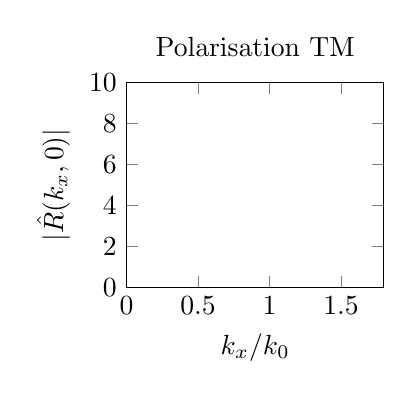
\begin{tikzpicture}[scale=1]
    \begin{axis}[
            title={Polarisation TM},
            ylabel={\(|\hat{R}(k_x,0)|\)},
            xlabel={\(k_x\slash k_0\)},
            width=0.4\textwidth,
            ymin=0,
            ymax=10,
            restrict y to domain=0:+4E+01,
            xmin=0,
            xmax=1.8,
            mark repeat=40,
            legend pos=outer north east
        ]
        % \addplot [color=black,mark=square*] table [col sep=comma, x={s1}, y={Abs(r_ex.tm)}] {csv/SOUDAIS/SOUDAIS.r_ex.MODE_2_TYPE_P.csv};
        % % \addlegendentry{Exact};

        % \addplot [color=blue,mark=x] table [col sep=comma, x={s1}, y={Abs(r_ibc0.tm)}] {csv/SOUDAIS/SOUDAIS.r_ibc.IBC_ibc0_SUC_F_MODE_2_TYPE_P.csv};
        % % \addlegendentry{CI0};

        % \addplot [color=red,mark=diamond*] table [col sep=comma, x={s1}, y={Abs(r_ibc3.tm)}] {csv/SOUDAIS/SOUDAIS.r_ibc.IBC_ibc3_SUC_F_MODE_2_TYPE_P.csv};
        % % \addlegendentry{CI3};
    \end{axis}
\end{tikzpicture}
\tikzsetnextfilename{R_SOUDAIS_plan_hoibc.TE}
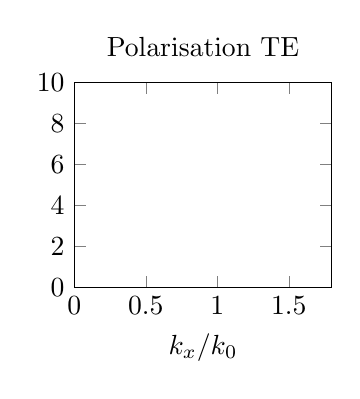
\begin{tikzpicture}[scale=1]
    \begin{axis}[
            title={Polarisation TE},
            ylabel={},
            xlabel={\(k_x\slash k_0\)},
            width=0.4\textwidth,
            xmin=0,
            xmax=1.8,
            ymin=0,
            ymax=10,
            mark repeat=40,
            legend pos=outer north east
        ]
        % \addplot [color=black,mark=square*] table [col sep=comma, x={s1}, y={Abs(r_ex.te)}] {csv/SOUDAIS/SOUDAIS.r_ex.MODE_2_TYPE_P.csv};
        % \addlegendentry{Exact};

        % \addplot [color=blue,mark=x] table [col sep=comma, x={s1}, y={Abs(r_ibc0.te)},color=] {csv/SOUDAIS/SOUDAIS.r_ibc.IBC_ibc0_SUC_F_MODE_2_TYPE_P.csv};
        % \addlegendentry{CI0};

        % \addplot [color=red,mark=diamond*] table [col sep=comma, x={s1}, y={Abs(r_ibc3.te)}] {csv/SOUDAIS/SOUDAIS.r_ibc.IBC_ibc3_SUC_F_MODE_2_TYPE_P.csv};
        % \addlegendentry{CI3};
    \end{axis}
\end{tikzpicture}
      %     \caption[CIOE sur empilement de P.~Soudais p.~11]{Module des coefficients diagonaux de \(\mR\) pour \(\eps = 4, \mu = 1, d=0.035\text{m}, f=12\text{GHz}\)}
      %     \label{fig:reflex_fourier:plan:soudais:hoibc}
      % \end{figure}

      Si la matrice d'impédance exacte possède plusieurs asymptotes, il faut autant de pôles à la CIOE pour être une bonne approximation.

      La figure \ref{fig:imp_fourier:plan:triple_asymptote:hoibc} montre la limite de la CI3 pour capturer trois asymptotes. Pour cela, il faudrait utiliser une CI d'ordre au moins 6 sur l'opérateur agissant sur \(\vE_t\). La CI3 n'est donc une bonne CIOE que si le nombre d'asymptotes est inférieur à 1, ce que l'on peut calculer connaissant l'empilement (voir proposition \ref{prop:imp_plan:symb_z:1c}).

      L'expression d'une CIOE vérifiant ce critère est la \hyperlink{ci7}{CI7}
      \begin{equation}
        \left(\oI + \sum_{i=1}^3 \left(d_{i} \left(\frac{\LD}{k_0^2}\right)^i + e_{i} \left(-\frac{\LR}{k_0^2}\right)^i \right)\right)\vE_t = \left(a_0 \oI + \sum_{i=1}^3 \left(b_{i} \left(\frac{\LD}{k_0^2}\right)^i + c_{i} \left(-\frac{\LR}{k_0^2}^i\right) \right)\right)\vJ.
      \end{equation}

      \begin{figure}[!hbt]
          \centering
          \tikzsetnextfilename{Z_triple_asymptote_plan_hoibc_TM}
\begin{tikzpicture}[scale=1]
    \begin{axis}[
            title={Polarisation TM},
            ylabel={\(\Im(\hat{Z}(k_x,0)\)},
            xlabel={\(k_x\slash k_0\)},
            width=0.4\textwidth,
            xmin=0,
            xmax=1.999,
            ymin=-10,
            ymax=10,
            restrict y to domain=-300:300,
            mark repeat=200,
            legend pos=outer north east
        ]
        \addplot [color=black,mark=square*] table [col sep=comma, x={s1}, y={Im(z_ex.tm)}] {csv/triple_asymptote/triple_asymptote.z_ex.P.csv};
        % \addlegendentry{Exact};

        \addplot [color=blue,mark=x] table [col sep=comma, x={s1}, y={Im(z_ibc0.tm)}] {csv/triple_asymptote/triple_asymptote.z_ibc.IBC_ibc0_TYPE_P_SUC_F.csv};
        % \addlegendentry{CI0};

        \addplot [color=red,mark=diamond*] table [col sep=comma, x={s1}, y={Im(z_ibc3.tm)}] {csv/triple_asymptote/triple_asymptote.z_ibc.IBC_ibc3_TYPE_P_SUC_F.csv};
        % \addlegendentry{CI3};

        \addplot [color=cyan,mark=pentagon*] table [col sep=comma, x={s1}, y={Im(z_ibc7.tm)}] {csv/triple_asymptote/triple_asymptote.z_ibc.IBC_ibc7_TYPE_P_SUC_F.csv};
        % \addlegendentry{CI7};
    \end{axis}
\end{tikzpicture}
\tikzsetnextfilename{Z_triple_asymptote_plan_hoibc_TE}
\begin{tikzpicture}[scale=1]
    \begin{axis}[
            title={Polarisation TE},
            ylabel={},
            xlabel={\(k_x\slash k_0\)},
            width=0.4\textwidth,
            xmin=0,
            xmax=1.999,
            ymin=-10,
            ymax=10,
            restrict y to domain=-300:300,
            mark repeat=200,
            legend pos=outer north east
        ]
        \addplot [color=black,mark=square*] table [col sep=comma, x={s1}, y={Im(z_ex.te)}] {csv/triple_asymptote/triple_asymptote.z_ex.P.csv};
        \addlegendentry{Exact};

        \addplot [color=blue,mark=x] table [col sep=comma, x={s1}, y={Im(z_ibc0.te)}] {csv/triple_asymptote/triple_asymptote.z_ibc.IBC_ibc0_TYPE_P_SUC_F.csv};
        \addlegendentry{CI0};

        \addplot [color=red,mark=diamond*] table [col sep=comma, x={s1}, y={Im(z_ibc3.te)}] {csv/triple_asymptote/triple_asymptote.z_ibc.IBC_ibc3_TYPE_P_SUC_F.csv};
        \addlegendentry{CI3};

        \addplot [color=cyan,mark=pentagon*] table [col sep=comma, x={s1}, y={Im(z_ibc7.te)}] {csv/triple_asymptote/triple_asymptote.z_ibc.IBC_ibc7_TYPE_P_SUC_F.csv};
        \addlegendentry{CI7};                  
    \end{axis}
\end{tikzpicture}
          \caption[CIOE sur empilement avec triple asymptote]{Partie imaginaire des coefficients diagonaux de \(\mZ\) pour \(\eps = 4, \mu = 1, d=0.2\text{m}, f=1\text{GHz}\)}
          \label{fig:imp_fourier:plan:triple_asymptote:hoibc}
      \end{figure}
      \begin{table}[!hbt]
        \centering
        \begin{minipage}[t]{0.49\textwidth}
        \vspace{0pt}
        \centering
        \begin{coefftable}{\hyperlink{ci0}{CI0}}
          \input{csv/triple_asymptote/triple_asymptote.IBC_ibc0_SUC_F_MODE_2_TYPE_P.coeff.txt}
        \end{coefftable}

        \begin{coefftable}{\hyperlink{ci3}{CI3}}
          \input{csv/triple_asymptote/triple_asymptote.IBC_ibc3_SUC_F_MODE_2_TYPE_P.coeff.txt}
        \end{coefftable}
        \end{minipage}
        \tablecoeff[0.49]{\hyperlink{ci7}{CI7}}{csv/triple_asymptote/triple_asymptote.IBC_ibc7_SUC_F_MODE_2_TYPE_P.coeff.txt}
        \caption{Coefficients associés à la figure \ref{fig:imp_fourier:plan:triple_asymptote:hoibc}}
        \label{tab:imp_fourier:plan:triple_asymptote:hoibc}
      \end{table}
